
\documentclass[twocolumn,11pt]{article}
\setlength{\textheight}{9truein}
\setlength{\topmargin}{-0.9truein}
\setlength{\parindent}{0pt}
\setlength{\parskip}{10pt}
\setlength{\columnsep}{.4in}
\newcommand{\beq}{\begin{equation}}
\newcommand{\eeq}{\end{equation}}
\renewcommand{\abstractname}{Abstract}
\usepackage{graphicx}
\usepackage{url}
\title{NAEST - Experiment 02 Report \\ Exploring U-Shaped Tubes: Investigating Confined Water Column Oscillations of Water in a U-Shaped Tube }
\author{Shuvam Banerji Seal\\2023WB00609}
\date{\today}
\usepackage{ragged2e}
\usepackage{amsmath}

\usepackage{mathtools}
\newtagform{dots}{\ldots(}{)}
\usepackage{amsfonts}
\usepackage{caption}
\usepackage{stackengine}
\usepackage{amssymb}
\usepackage{graphicx}
\usepackage{accents}
\usepackage{booktabs}
\usepackage{eqnarray}
\usepackage{url}
\usepackage{blindtext}
\usepackage{tcolorbox}
\usepackage{graphicx}   
\usepackage{amsthm}
\usepackage{algorithm}
\usepackage{hyperref}
\hypersetup{
    colorlinks=true,
    linkcolor=blue,
    filecolor=magenta,      
    urlcolor=blue,
    pdftitle={NAEST-Shuvam Banerji Seal},
    pdfpagemode=FullScreen,
    }
\usepackage{gensymb}
\usepackage{algpseudocode}
\usepackage{subcaption}
\usepackage[english]{babel}
\usepackage[export]{adjustbox}
\usepackage{enumerate}
\usepackage[left=2.5cm,right=2.5cm,top=1.5cm,bottom=1.5cm]{geometry}
\usepackage{lineno}
\usepackage{cite}
\usepackage{acronym}
\usepackage{xcolor}
\newcommand{\remark}[3]{%
    {\colorbox{#2}{\sffamily\scriptsize\bfseries\textcolor{white}{#1}}}
    {\sffamily\small\itshape\textcolor{#2}{#3}}
}

\begin{document}
\definecolor{aqua}{rgb}{0.0, 1.0, 1.0}
%\hypersetup{colorlinks,urlcolor=blue}
\pagestyle{plain}
 \twocolumn[
   \begin{@twocolumnfalse}
   \textbf{\maketitle}
   \setlength{\parindent}{0pt}
   \begin{abstract} 
   \textbf{Keywords:} oscillatory behavior, water column, U-shaped tube, simple harmonic motion, energy dissipation, acceleration due to gravity, tube diameter.
\vspace{0.5cm}
This experiment investigates the oscillatory behavior of a water column confined within a U-shaped tube to analyze parameters related to simple harmonic motion and energy dissipation. The study aims to determine the acceleration due to gravity ($g$) and explore the effects of tube diameter on the oscillation characteristics. The experiment involves measuring the time period of oscillation for different lengths of the water column in two tubes with varying diameters. The results show that the average values of $g$ for the thicker and thinner tubes are $853.56\,cm/sec^2$ and $1033.6\,cm/sec^2$ respectively. The experiment also quantifies the rate of energy dissipation, which is influenced by factors such as viscosity, friction, and turbulence. A comparative analysis between the two tubes reveals differences in the observed $g$ values due to diameter-related effects and energy dissipation variations. The experiment highlights the importance of considering these factors in oscillatory systems. Despite limitations such as potential measurement errors and variations in oscillation amplitude, the study provides valuable insights into the complex interplay between simple harmonic motion, fluid properties, and tube geometry. 



		\vspace{.3in} 
     \end{abstract}
    \end{@twocolumnfalse}]


\section{Introduction}
A manometer is a useful device for measuring the pressure of liquids and gases. In this experiment, the aim is to construct a water manometer and investigate the oscillations of a water column inside it. The setup involves two transparent and flexible plastic pipes with different diameters to form a U-tube. By studying the oscillations and measurements, we will gain insights into the behavior of the water column and its relationship with length and time period.

\section{Theory}
\subsection{Oscillations in a U-tube Manometer}
When a water column is confined within a U-tube manometer and subjected to a disturbance, such as a sudden change in water level, the water column undergoes oscillations. The oscillations are periodic, and their frequency is determined by the length of the water column and the acceleration due to gravity.

\subsection{Period of Oscillation ($T$)}
The time period ($T$) of the oscillation refers to the time taken for the water column to complete one full oscillation. It can be measured by observing the time taken for the water column to return to its initial position after being displaced.

\subsection{Oscillation Damping}
During oscillations, the energy of the water column is gradually dissipated due to various factors, including viscosity, friction, and turbulence. As a result, the amplitude of oscillation decreases over time until the water column comes to rest.

\subsection{Effective Acceleration due to Gravity ($g$)}
The period of oscillation ($T$) is related to the effective acceleration due to gravity ($g$) and the entire length of the water column ($L$) by the formula:
\begin{equation}
\label{Equation for Time Period}
\usetagform{dots}
T = 2\pi\sqrt{\frac{L}{2g}}
\end{equation}
 By measuring $T$ for different lengths $L$, we can determine the effective value of $g$ for the oscillating system, using
 \begin{equation}
     \label{Working Formula for g}
     \usetagform{dots}
     g= \frac{2 \pi^2 L }{T^2}
 \end{equation}



\subsection{Viscosity of Water}
Viscosity plays a role in the oscillations of the water column by affecting the dissipation of energy. Higher viscosity results in more damping, leading to shorter oscillation periods and impacting the value of $g$ obtained.

\section{Materials Required}

To conduct this experiment, we will require the following materials:
\begin{itemize}
    \item Water
    \item Scales \footnote{I used a metal, instead of a plastic one, as that was what was available in my stuff at the hostel.}
    \item Transparent flexible Tubes\footnote{It was very difficult for me to get it, since my campus feels like it's in the middle of nowhere. And I had to separately buy it, sadly.} 
    \item Small Rubber balls/ anything that can cover the top end of the tube and thus making it airtight.
    \item Stopwatch or mobile with a timer function
    \item Camera/ Mobile videography so that accurate data of the time period can be acquired and also to capture the videos of the experimental procedure (as asked in the problem statement)
\end{itemize}

\section{Understanding the Process}
\subsection{Making the Manometer}
\begin{itemize}
    \item Procure two transparent and flexible plastic pipes with diameters of approximately 1.27cm(0.5 inch) and 2.54cm (1 inch)\footnote{The reason that I am saying the diameters with confidence is because these were factory made and were the sizes available (costed me 200 INR... sad life)} and lengths around 2 meters.
    \item Create a U-shape with the thicker pipe and attach it vertically to a cupboard or wall.
    \item Ensure most of the pipe (excluding the curved bottom end) is vertical for accurate measurements.
    \item Set up a measurement scale to quantify water levels in the U-tube.
\end{itemize}

\subsection{Part 1.a: Oscillations of Water Column in Thicker Pipe}
\begin{itemize}
    \item Fill approximately 30cm of water into the thicker pipe.
    \item Close one end of the pipe with a rubber ball\footnote{I again wasn't able to source it, so the experiment was done using the palm of our hands to make an airtight seal.}, ensuring an airtight seal.
    \item Measure the length of the trapped air column between the closed end and the water surface (should be more than 50cm).
    \item Pour additional water into the open end of the tube and note the height difference between the water levels in both arms.
    \item Remove the rubber ball, causing the water column to oscillate.
    \item Measure the time period ($T$) of oscillation for this length of the water column.
    \item Repeat the procedure, changing the length of the water column each time by adjusting the water levels.
    \item Record the time periods ($T$) and the number of oscillations before damping.
\end{itemize}
\subsection{Part - 1.b : Understanding from the slopes}
\begin{itemize}
    \item Find the slope of the straight line between $T^2$ vs $L$ (the straight line passes through the origin).

    \item Calculate terrestrial acceleration from the relation, 
    \begin{equation}
    \label{G from slope}
    \usetagform{dots}
    g = \dfrac{2\pi^2}{\text{slope}}.        
    \end{equation}    
 \end{itemize}

\section{Calculations and Data Tabulation:}
\subsection{Part 1.a: Data Table to Tabulate the time intervals of Oscillations of water in the Thick (2.54cm diameter) Tube}
\subsubsection{Length Data of the water column}
\begin{center}
\begin{tabular}{||p{0.5cm} | p{2cm}| p{2cm}| p{2cm} ||} 
 \hline
 SL. No. & Water level Difference between the two columns (cm) & Length of the water column in the U-shaped const. region(cm) & Total Length of the water Column (cm) ||\\ 
 \hline\hline
 1 & 43.5 & 100 & 143.5 \\ 
 \hline
 2 & 49.5 & 70 & 119.5 \\
 \hline
 3 & 66 & 73 & 139\\
 \hline
 4 & 22 &  98 & 120 \\
 \hline
 5 & 22 & 119 & 141  \\ 
 \hline
 6 & 30 & 151 & 181\\
 \hline
  7 & 54 & 76 & 130\\
 \hline
  8 & 96.5 & 27.5 & 124\\
 \hline
  9 & 105 & 29 & 134\\
 \hline
  10 & 78 & 47 & 125\\
 \hline
  11 & 30 & 107 & 137\\
 \hline
  12 & 22.5 & 127.5 & 150\\
 \hline
  13 & 90 & 65 & 153\\
 \hline
 \hline
\end{tabular}
\end{center}


\subsubsection{Time-Period Data Table}

\begin{center}
\begin{tabular}{||p{0.5cm} | p{1.5cm}| p{1.5cm}| p{0.5cm} |p{2cm}||} 
  \hline
 SL. No. & Total Length of the water Column (cm) & Total Time of Oscillations (sec) & No. of Oscillations & Average Time Period [Total time/ No. of Oscillations] (sec) \\ [0.5ex] 
 \hline\hline
 1 & 143.5 & 13.694 & 7 & 1.956 \\ 
 \hline
 2 & 119.5 & 13.123 & 6 & 1.793 \\
 \hline
 3 & 139 & 16.930 & 9 & 1.881\\
 \hline
 4 & 120 & 13.218 & 9 & 1.469 \\
 \hline
 5 & 141 & 17.817 & 10 & 1.782\\ 
 \hline
 6 & 181 & 19.732 & 10 & 1.973\\ 
 \hline
 7 & 130 & 15.203 & 8 & 1.900\\ 
 \hline
 8 & 124 & 14.527 & 8 & 1.816\\ 
 \hline
 9 & 134 & 15.968 & 9 & 1.774\\ 
 \hline
 10 & 125 & 14.697 & 9 & 1.633\\ 
 \hline
 11 & 137 & 16.489 & 10 & 1.649\\ 
 \hline
 12 & 150 & 18.287 & 10 & 1.829\\ 
 \hline
 13 & 153 & 18.777 & 10 & 1.878\\ 
 \hline
 \hline
\end{tabular}
\end{center}


\subsubsection{Calculating The Acceleration due to Gravity ($g$)}
\begin{figure}[H]
    \centering
    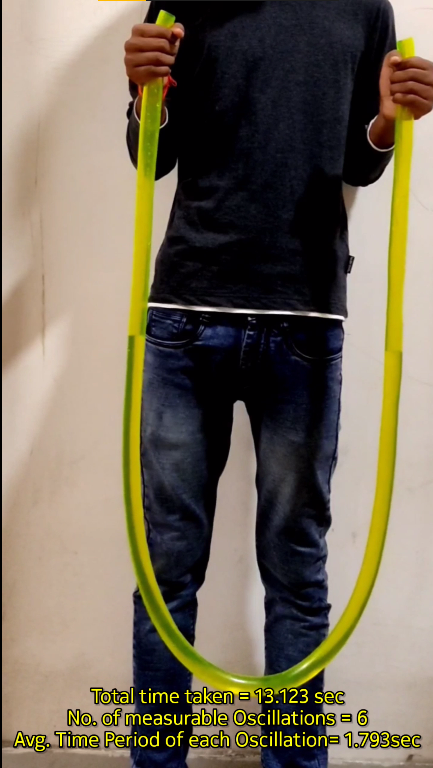
\includegraphics[scale =0.4]{abhinandan-holding pipe.png}
    \caption{Set-up and experimental measurements. Click \href{https://drive.google.com/file/d/1sTAGJjE_yXGOSd3VcdA2fcaamWB1AhRL/view?usp=drive_link}{here} for the measurement video demostration}
    \label{Video_demo_abinandan}
\end{figure}
    Note: Only three data-taking events\footnote{And I want to thank my hostel friends who helped me to get the measurements for this experiment} are shown due to the time limit, but all the others are done in the same manner. 
    
    Next, let's calculate the values of $g$ we get from the whole data set using \eqref{Working Formula for g},


\begin{center}
\begin{tabular}{||p{0.5cm}||p{1.5cm}|p{2cm}| p{2cm}||} 
 \hline
 SL. No. & Length of the Entire Water Column (cm) & Average Time Period (sec) & Acceleration due to gravity ($g$)(cm/sec^2) \\ [0.5ex] 
 \hline\hline
 1 & 143.5  & 1.956 & 740.4\\ 
 \hline
 2 & 119.5  & 1.793 & 733.7\\
 \hline
 3 & 139  & 1.881 & 775.5\\
  \hline
  4 & 120 & 1.469  & 1097.7\\
 \hline
 5 & 141 & 1.782 & 876.5\\ 
 \hline
 6 & 181 & 1.973 & 917.8\\ 
 \hline
 7 & 130 & 1.900 & 710.8\\ 
 \hline
 8 & 124 & 1.816 & 742.2\\ 
 \hline
 9 & 134 & 1.774 & 840.5\\ 
 \hline
 10 & 125 & 1.633 & 925.3\\ 
 \hline
 11 & 137 & 1.649 & 994.5\\ 
 \hline
 12 & 150 & 1.829 & 885.1\\ 
 \hline
 13 & 153 & 1.878 & 856.3\\ 
 \hline
 \hline
\end{tabular}
\end{center}

So, from all the values of $g$, the average $g$ that we got experimentally is,
\begin{equation}
    \label{Average g from Thicc Pipe}
 \usetagform{dots}
    g =  853.56  cm/sec^2
\end{equation}

\subsection{Part 1.b: Repeating the same Experimental Procedure for the tube of 1.27cm Diameter}
\subsubsection{Length Data of the water column}
\begin{center}
\begin{tabular}{||p{0.5cm} | p{2cm}| p{2cm}| p{2cm} ||} 
 \hline
 SL. No. & Water level Difference between the two columns (cm) & Length of the water column in the U-shaped const. region(cm) & Total Length of the water Column (cm) ||\\ 
 \hline\hline
 1 & 66 & 71.5 & 137.5 \\ 
 \hline
 2 & 75 & 55 & 130 \\
 \hline
 3 & 53.5 & 73 & 126.5\\
 \hline
 4 & 47.3 &  116.5 & 163.8 \\
 \hline
 5 & 40 & 157.5 & 197.5  \\ 
 \hline
 6 & 29 & 161 & 190\\
 \hline
 \hline
\end{tabular}
\end{center}

\subsubsection{Time-Period Data Table}

\begin{center}
\begin{tabular}{||p{0.5cm} | p{1.5cm}| p{1.5cm}| p{0.5cm} |p{2cm}||} 
 \hline
 SL. No. & Total Length of the water Column (cm) & Total Time of Oscillations(sec) & No. of Oscillations & Average Time Period [Total time/ No. of Oscillations] (sec) ||\\ [0.5ex] 
 \hline\hline
 1 & 137.5 & 12.457 & 8 & 1.557 \\ 
 \hline
 2 & 130 & 10.188 & 6 & 1.698 \\
 \hline
 3 & 126.5 & 13.337 & 8 & 1.667\\
 \hline
 4 & 163.8 & 21.344 &12 & 1.778 \\
 \hline
 5 & 197.5 & 18.838 & 10 & 1.884\\
 \hline
 6 & 190 & 19.963 & 11 & 1.815 \\
 \hline
 \hline
\end{tabular}
\end{center}


\subsubsection{Calculating The Acceleration due to Gravity ($g$)}

    Next, let's calculate the values of $g$ we get from the whole data set using \eqref{Working Formula for g},

\begin{center}
\begin{tabular}{||p{0.5cm}||p{1.5cm}|p{2cm}| p{2cm}||} 
 \hline
 SL. No. & Length of the Entire Water Column (cm/sec) & Time Period (sec) & Acceleration due to gravity ($g$)(cm/sec^s) \\ [0.5ex] 
 \hline\hline
  1 & 137.5 & 1.557 & 1119.6\\ 
 \hline
 2 & 130  & 1.698 & 923.4\\
 \hline
 3 & 126.5  8 & 1.667 & 898.6\\
 \hline
 4 & 163.8  & 1.778 &1022.8\\
 \hline
 5 & 197.5  & 1.884 & 1098.3\\
 \hline
 6 & 190  & 1.815 & 1138.5\\
 \hline

 \hline
\end{tabular}
\end{center}

So, from all the values of $g$, the average $g$ that we got experimentally is,
\begin{equation}
    \label{Average g}
 \usetagform{dots}
    g =  1033.6  cm/sec^2
\end{equation}
\subsection{A Final Average?(Let's do it)}
The only reason that I am doing another average of the two acceleration due to gravity values from the two pipes, is just to reduce the randomness of human mistakes and the envirnmental influences. Let's do it then.
\begin{equation}
    \label{Final g}
    g_{final\_avg} = \frac{1033.6 + 853.5}{2} = 943.6 cm/sec^2
\end{equation}
\begin{figure}[H]
    \centering
    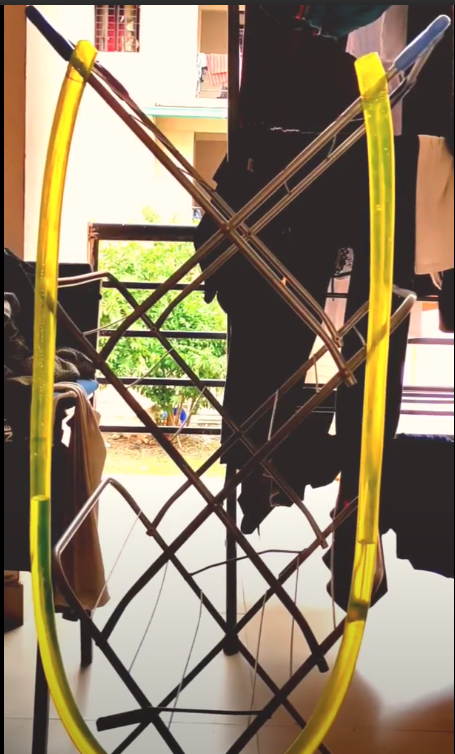
\includegraphics[scale =0.4]{new_setup.png}
    \caption{A new-setup where majority of the data collection was done. But I wasn't able to create a specific video for it. I am just attaching a simple video to better show the data collection process. See \href{https://drive.google.com/file/d/1B0Kj0nX2NHbx1PAJz2C6tWp1hRgPLPga/view?usp=sharing}{Video.} }
    \label{Video_demo_new_setup}
\end{figure}

\section{Plotting the Graphs:}
The Graphs are plotted for both the pipes, but sadly, though, I was able to get 13 data points for the 2.54cm diameter one which is quite a lot when compared to the thin 1.27 cm diameter pipe\footnote{I wasn't able to hold on to my friends for long enough to collect a few more data points for this. Sadly, our college never lets us to even breathe.}. 

\begin{tcolorbox}[width=8cm,colback={aqua},title={Note 01},colbacktitle=white,coltitle=black]    
    I have added the .gnu scripts, the log file of the fitting and also the plots in the drive. Click \href{https://drive.google.com/drive/folders/1RKSEggA8p61pM14YIgWOVmSHRRIRab_b?usp=sharing}{here} to view.
\end{tcolorbox}

\begin{tcolorbox}[width=8cm,colback={aqua},title={Note 02},colbacktitle=white,coltitle=black]    
    For accuracy, I need some form of support to hang the pipes, which I later got and from that rack only I took most of the data points. See \href{https://drive.google.com/file/d/1B0Kj0nX2NHbx1PAJz2C6tWp1hRgPLPga/view?usp=drive_link}{Video} for refernce.
\end{tcolorbox}

\subsection{$T^2$ v/s $L$ plot (Thick pipe):}
\begin{figure}[H]
    \centering
    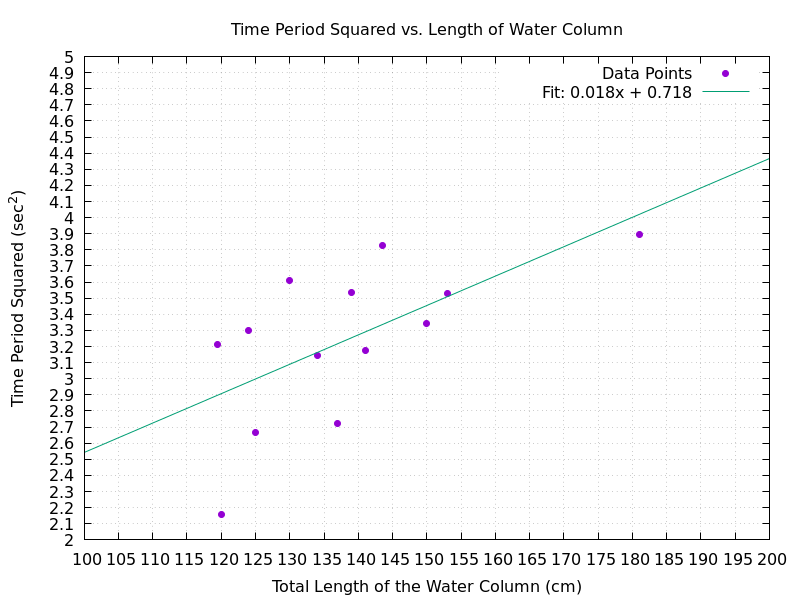
\includegraphics[scale=0.3]{T2_vs_L.png}
    \caption{The $T^2$ vs L plot for the thicker pipe. Notice that the slope is 0.018. We will be using this.}
    \label{T2_vs_L}
\end{figure}
\subsection{$T^2$ v/s $L$ plot (Thin Pipe):}
\begin{figure}[H]
    \centering
    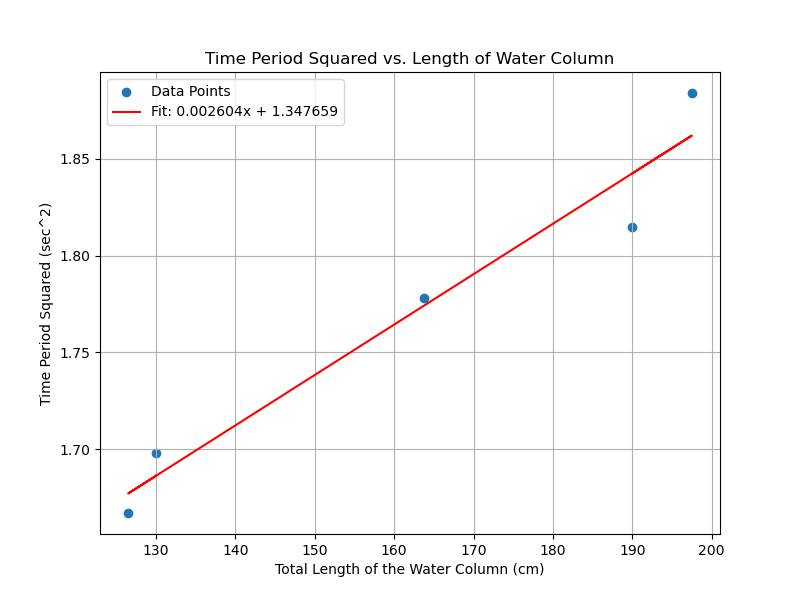
\includegraphics[scale=0.4]{T2L using matplotlib.png}
    \caption{The $T^2$ vs L plot for the thicker pipe. Notice that the slope is 0.0026, which is a whole order of magnitude different.We shall later be discussing it.}
    \label{T2_vs_L}
\end{figure}
\subsubsection{Extra : Finding the Value of $g$ Using the plot:}
Refer \eqref{G from slope},\\
Using the Slope = 0.018, we can again check for the value of g,
Putting the value of the slope in \eqref{G from slope}, we get
$$g_{slpoe} = \frac{2\pi^2}{Slope} = 1096.6 cm/sec^2$$
\subsection{$T$ v/s $L$ plot(Thick Pipe):}
\begin{figure}[H]
    \centering
    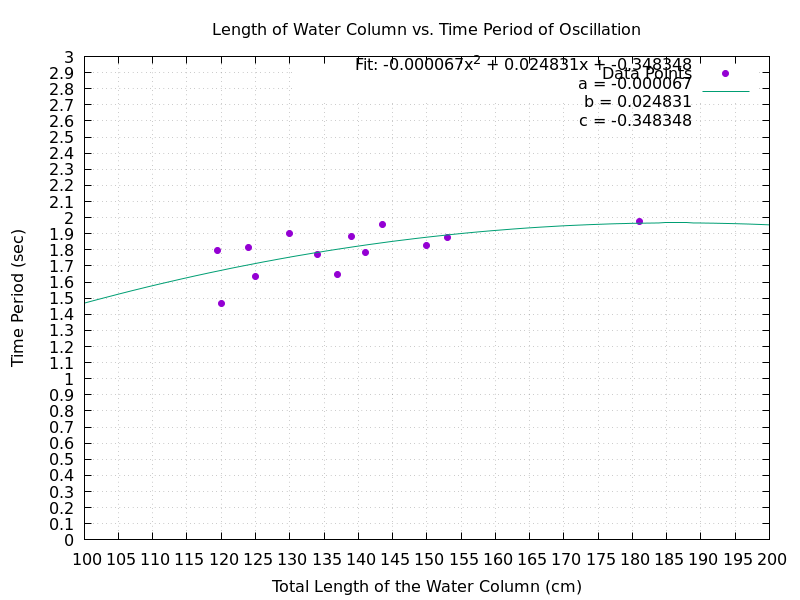
\includegraphics[scale=0.3]{L_vs_T.png}
    \caption{The $T$ vs L plot for the thicker pipe}
    \label{T2_vs_L}
\end{figure}
\subsection{$T$ v/s $L$ plot (Thin pipe):}
\begin{figure}[H]
    \centering
    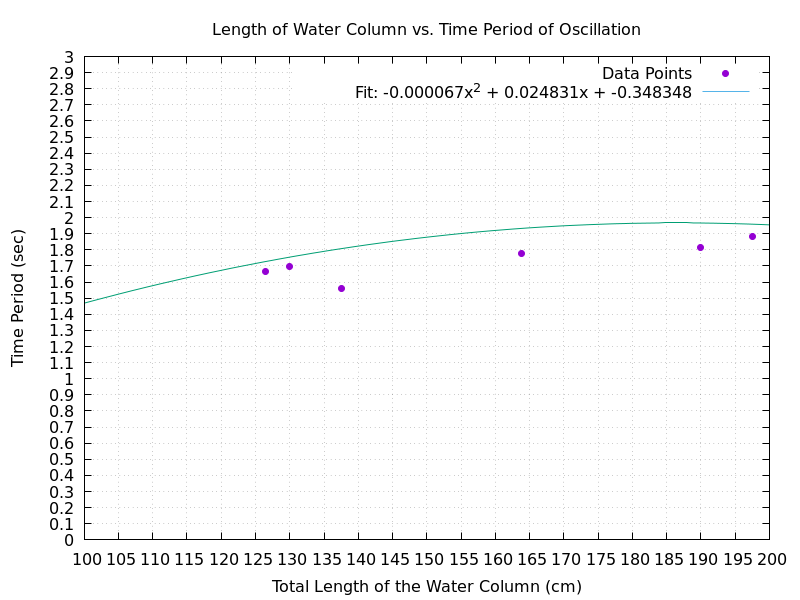
\includegraphics[scale=0.3]{L_vs_T_Thin_pipe.png}
    \caption{The $T$ vs L plot for the thin pipe of diameter 1.27cm}
    \label{T2_vs_L}
\end{figure}

\section{Part 2: Average rate of dissipation of energy}

\subsection{The Derivation of the Working Formulae:(\textbf{Extra})}
\begin{figure}[H]
    \centering
    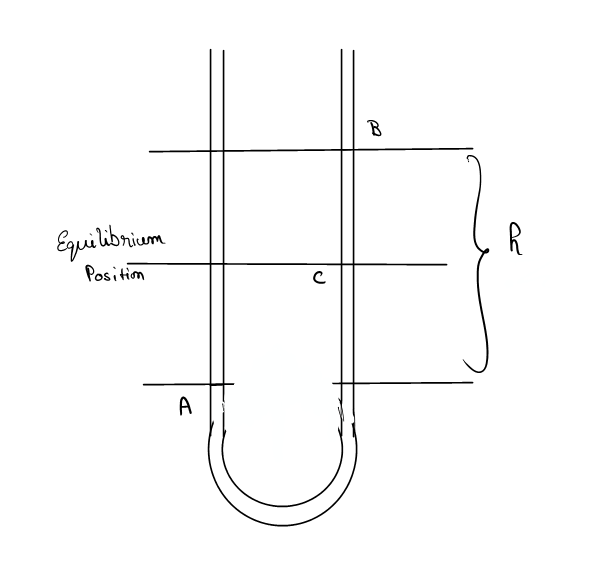
\includegraphics[scale =0.6]{U-tube_Illustrations.png}
    \caption{An illustration for the derivation}
    \label{U-tube illustration}
\end{figure}

For the derivation of the expression that I will be using to calculate the Average energy dissipation rate, first, let's find the energy that causes the oscillations.

P - Pressure of the water\\
$\rho$ - density of the water, and today was 27\degree C so, $\rho = 0.996512 gm/cc$, Refer \cite{density_of_water_0-100_Celsius}\\
$A$- Area of the cross-section of the tube\\
$h$ - Height difference between the two water levels\\
The Energy that does the work =  Total Energy stored - The Energy terms which don't contribute


\begin{equation}
    \label{The extra energy}
   U &= \frac{1}{2} (h + \frac{P}{g \rho})^2 - \frac{1}{2}(\frac{P}{g \rho})^2\rho Ag - \frac{1}{2}\rho h^2A   
\end{equation}
$= PAgh$\\
Now, replacing $P= h\rho g$, we get,
\begin{equation}
    \label{Working formula for energy extra}
    = \rho h^2 g A
\end{equation}
\begin{tcolorbox}[width=8cm,colback={aqua},title={A more simpler derivation},colbacktitle=white,coltitle=black]    
   Observe that the oscillations are only caused by the store potential energy stored in the higher water column, and we know that potential energy at some height h is $mgh$, where $m = \rho A h$,
   so,
   \begin{equation}
       \label{Extra energy simple}
       U = \rho A h^2 g
   \end{equation}

\end{tcolorbox}
Now, knowing that \\
$n = \text{No. of Oscillations}$\\
$T_{total} = $Total time interval for each case till the last observable measurement made.\\
From both \eqref{The extra energy} and \eqref{Extra energy simple}, we get the Final rate of dissipation of energy ($D_{avg}$), as
\begin{equation}
    \label{Rate of Energy Dissipation}
    D = \frac{\rho Ah^2g}{T}
\end{equation}
So,
\begin{equation}
    \label{Avg Rate of Energy Dissipation}
    D_{avg} = \sum_{i=1}^{10} \frac{\rho Ah_i^2g}{10T_i}
\end{equation}
\subsection{Tabulating the Data for Thick pipe}


\begin{center}
\begin{tabular}{||p{0.5cm} | p{1cm}| p{1.5cm}| p{1.3cm} | p{2cm}||} 
 \hline
    SL. No. & g $(cm/sec^2)$ & Total Time of Oscillations(sec) & Height of the water column (h)(cm) & Energy Dissipated (D) (Joule) ||\\ [0.5ex] 
 \hline\hline
 1 & 740.4 & 13.694 & 43.5 & 0.052\\ 
 \hline
 2 & 733.7 & 13.123 & 49.5 & 0.069 \\
 \hline
 3 & 775.5 & 16.930 & 66 & 0.1\\
 \hline
 4 & 1097.7 & 13.218 & 22 & 0.02\\
 \hline
 5 & 876.5 & 17.817 & 22 & 0.012\\
 \hline
 6 & 917.8 & 19.732 & 30 & 0.021\\
 \hline
 7 & 710.8 & 15.203 & 54 & 0.069\\
 \hline
 8 & 742.2 & 14.527 & 96.5 & 0.2\\
 \hline
 9 & 840.5 & 15.968 & 105 & 0.3\\
 \hline
 10  & 925.3 & 14.697 & 78 & 0.2\\
 \hline
 11 & 994.5 & 16.489 & 30 & 0.027\\
 \hline
 12 & 885.1 & 18.287 & 22.5 & 0.012\\
 \hline
 13 & 856.3 & 18.777 & 90 & 0.186\\
 \hline
 \hline
\end{tabular}
\end{center}

Now, coming to $D_{avg}$ we get,
\begin{equation}
    \label{avg. rate of energy diddipation for thick tube}
    D_{avg} = 0.0976 J/sec
\end{equation}
Since, we are talking about dissipation, the $D_{avg}$ must be negative, but here only the magnitude of the average rate of dissipation of energy is talked about. 

\subsection{Tabulating the Data for Thin (radius = 0.635cm) pipe}


\begin{center}
\begin{tabular}{||p{0.5cm} | p{1cm}| p{1.5cm}| p{1.3cm} | p{2cm}||} 
 \hline
    SL. No. & g $(cm/sec^2)$ & Total Time of Oscillations(sec) & Height of the water column (h)(cm) & Energy Dissipated (D) (Joule) ||\\ [0.5ex] 
 \hline\hline
 1 & 1119.6 & 12.457 & 66 & 0.05\\ 
 \hline
 2 & 923.4 & 10.188 & 75 & 0.064 \\
 \hline
 3 & 898.6 & 13.337 & 53.5 & 0.024\\
 \hline
 4 & 1022.8 & 21.344 & 47.3 & 0.014\\
 \hline
 5 & 1098.3 & 18.838 & 40 & 0.012\\
 \hline
 6 & 1138.5 & 19.963 & 29 & 0.006\\
 \hline

 \hline
 \hline
\end{tabular}
\end{center}

Now, coming to $D_{avg}$ we get,
\begin{equation}
    \label{avg. rate of energy diddipation for thin tube}
    D_{avg} = 0.028 J/sec
\end{equation}
Since, we are talking about dissipation, the $D_{avg}$ must be negative, but here only the magnitude of the average rate of dissipation of energy is talked about. 


\begin{comment}
    

\section{Some Theoretical Discussions}    
\end{comment}

\section{Final Observation, Comparison and Thoughts: (along with something extra)}
If we were to compare the outcomes of the two environments for the simple harmonic motion to occur in the case of water, theoretically the thickness of the tube should not matter, but "reality is stranger than fiction".
\subsection{Density Dependence:}
\begin{figure}[h]
    \centering
    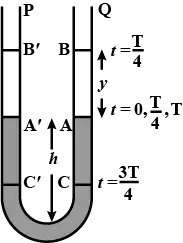
\includegraphics[scale=0.7]{SHM_no_density.png}
    \caption{Illustration for the given derivation}
    \label{fig:enter-label}
\end{figure}

Consider a U-tube filled with a liquid of density $\rho$ up to height $h$ as shown in the figure. When the liquid is lifted up to a height $y$ from A to B in arm Q, the liquid level in arm P drops by $y$ from A to C, with the height difference between the two arms given by $2y$. Then the force $F = -\rho gA(2y)$, where $F=ma=(2LA\rho)$, so the acceleration is ...
$$a =- \frac{2yA\rho g}{\rho LA}$$

\begin{equation}
    \label{exp for acc}
    a= -\frac{2g}{L}y
\end{equation}
Again, as the motion is SHM, we know that
\begin{equation}
    \label{shm ACC exp}
    a = - \omega^2 y
\end{equation}

The motion of an oscillating liquid column in a U-tube is Simple Harmonic Motion (SHM) with a period $T = 2\pi \sqrt{\dfrac{L}{2g}}$, where $L$ is the total length of the water column in its equilibrium position. Therefore, $T$ is independent of the density of the liquid.

\subsection{Effect of Damping}
Comparing \eqref{exp for acc} and \eqref{shm ACC exp}, we get,
\begin{equation}
    \label{omegha}
    \omega^2 = \frac{k}{m} = \frac{2g}{L}
\end{equation}
where k is the constant related to the reluctness of the fluid to show motion, $m$ is the mass of the liquid that starts the oscillation.

Again, since this is a real-life case, there will be of course some amount of damping, let's assume that the damping comes as the first differential of motion, ie a velocity term. 
\begin{equation}
    \label{Differential eq for damped shm}
    m\ddot x +b \dot x + kx = 0
\end{equation}

Solving \eqref{Differential eq for damped shm}, will reveal,

\begin{equation}
    \label{omega damped}
    \omega = \sqrt{\frac{k}{m}-\frac{b}{2m}^2}
\end{equation}
Now putting the expression for $\frac{k}{m}$ from \eqref{omegha}, in \eqref{omega damped}, we get the following,
$$b = \sqrt{4m^2(\frac{2g}{L}-\frac{4\pi^2}{T^2})}$$
Again we can write the mass as,
$$m= \text{Density}\times \text{Volume}$$

$$m = \rho V = \rho (\pi R^2 h)$$

And so finally we get the damping constant $b$, as
\begin{equation}
    \label{damping constant}
    b = 2\rho \pi R^2 h \sqrt{\frac{2g}{L}-\frac{4\pi^2}{T^2}}
\end{equation}

Now calculating b for the thick pipe for a few value (taken at random), gives
$${b_{2.54cm\_diameter}}_{avg\_for\_first\_three\_values} $$$$= 815.4 dyne\frac{sec}{cm}$$

Now like the mathematics books, I am going to leave finding the average damping constant for the thin pipe to the reader as an exercise. 
\\
Again the existence of this damping constant also shows that the time period of each oscillation should be greater than their theoretical counter-part, and that the energy dissipated would be greater than what we calculated (Remember in ideal undamped case, oscillations would go on till infinity, as no energy gets lost from the system) 

\subsection{Energy Dissipation Phenomenon(considering damping to exist)}
From the previous section, I have already derived the expression for damping, and trivial from that and \eqref{Differential eq for damped shm}, we can say,
$$E_o = \text{Energy in undamped oscillations}$$
$$E_d = \text{Energy in damped oscillations}$$
\begin{equation}
    \label{energy ini damping}
    E_d = E_d \exp{\frac{-bt}{2m}}
    \end{equation}

Now, from \eqref{damping constant} and \eqref{energy ini damping}, we can more accurately gauge the energy dissipated per unit time and also the average rate at which it does it.

\section{Error Analysis :}
\subsection{Systematic/Instrumental Error Analysis:}

    We need to note that the errors are here only with respect to the least count of the instrument used.

    Refer \eqref{Working Formula for g}, now to find the instrumental error bounds we first take log and then differentiate while considering cumulative nature of error,

\begin{equation}
    \label{theoritical error expression}
    \frac{\Delta g}{g} = \frac{\Delta L}{L} + 2\frac{\Delta T}{t}
\end{equation}


Note: Here the length corresponds to the length measured by the 30cm scale with a Least Count of 0.1cm and for the Time Interval, I used the software to get the almost exact frame where I released the hand, and there, the least count was 0.001 secs based on the frame-rate and interpolation of the camera software.\\

Again, as there are different lengths and intervals co-responding to different measurements, let me just pick some random data row (say 3 from the Time-period data Table for 2.54cm diameter tube),

Therefore,
$$\frac{\Delta g}{g} = \frac{0.1}{139} + 2\frac{0.001}{1.881}=1.78 \times 10^{-3}$$

So, for some random data row, we are getting the instrumentational error at the order of 0.1\%, which is quite less.

    


\subsection{Relative Error Calculation wrt Literature Values:}
The value of acceleration due to gravity $g$ is very well known. With regional variability in mind, the value of $g=980cm/sec^2$ in my current place of residence. The value after three significance digits changes due to various reasons (let's not get into that).

What I can now do is to check how off we are from the actual value.
Refer \eqref{Final g}, as I shall be using this as the final experimental result to compare with the theoritical/actual value.

Again, so,

$$\text{Relative Error \%} =$$
\begin{equation}
\label{Relative_Error}
\frac{|Observed Value-Literature Value|}{Literature Value} \times 100 \%
\end{equation}
$$=\frac{|980-943.6|}{980} \times 100 \%$$
$$=3.71\%$$
\subsection{Standard Deviation for $g$:}

I have created a python code to plot the standard deviation data using matplot to get the visual representation of how the experimental values are distributed.

On the Vertical axis, I named it "Probability Density", as it represented that if someone else woould replicate my experimental set-up, then the chance of him or her getting the sane nature of data points.

The figure would be self-explainatory with the values printed.

\begin{figure}[H]
    \centering
    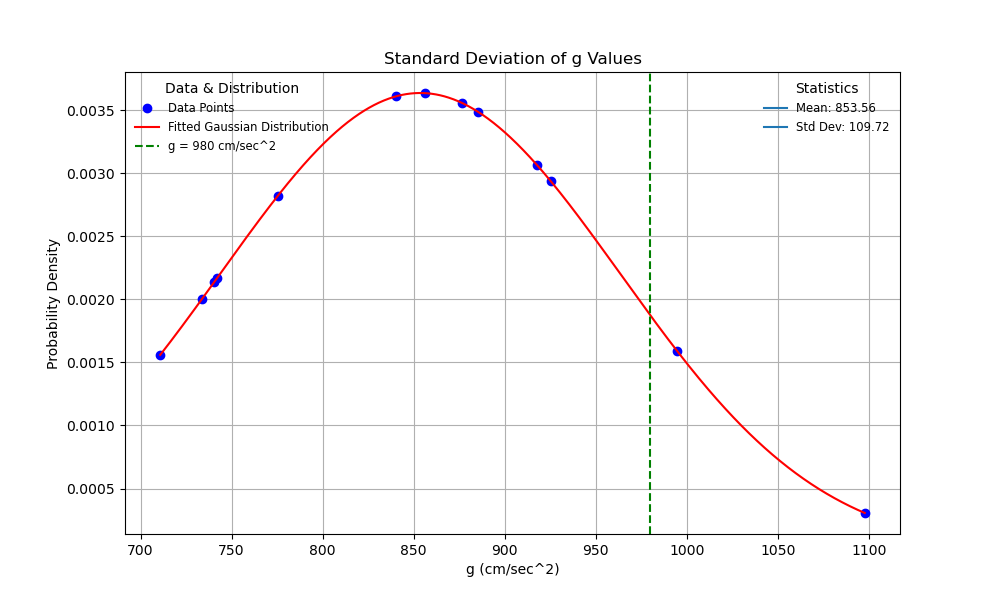
\includegraphics[scale = 0.35]{std_dev_plot_thick.png}
    \caption{Standard deviation plot for the 2.54cm diameter pipe. Here, standard deviation = $109.72cm/sec^2$ }
    \label{fig:enter-label}
\end{figure}

\begin{figure}[H]
    \centering
    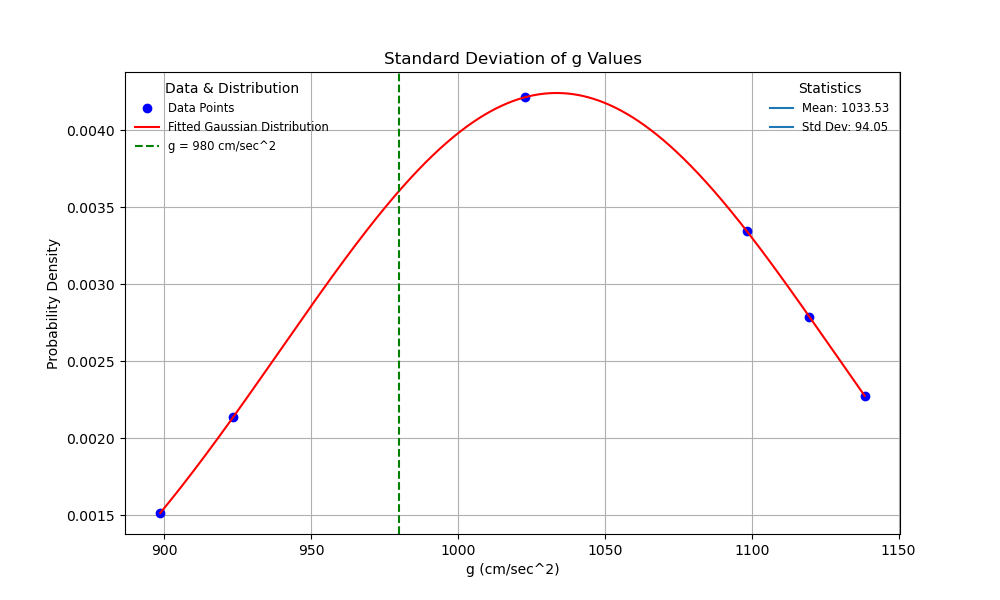
\includegraphics[scale = 0.35]{std_dev_plot_thin.png}
    \caption{Standard deviation plot for the 1.27cm diameter pipe. Here, standard deviation = $94.05cm/sec^2$ }
    \label{fig:enter-label}
\end{figure}

\subsubsection{For the Thick pipe(2.54cm diameter)}
\section{Sources of Error:}
First of all, conducting this experiment was very difficult\footnote{due to various reasons like unavailability of the pipes, to not so suitable places to stage the pipes, and most of all the requirement of a friend, though not totally necessary but it really speeds up the process} but whatsoever, it was fun nonetheless. 
\\
Now coming back to the sources of error, they are explained as follows:
\begin{enumerate}
    \item The Flexible plastic pipe was very sticky with some form of latex spread over it to prevent it from drying up. But then again, I have no idea how this affects the flow of the water as it passes through it, like the magnitude of adhesive forces, etc.
    \item The equations used here are for undamped oscillators but the real and daily life apparatus that we are using, they are not that ideal and some energy will always get lost.
    \item After the sealed end of the tube is opened, whether it's a human holding it or being hung from some point, the whole tube sways quite a bit. This will of course disturb the ongoing simple harmonic motion and thus may result in erroneous outcomes.
    \item Also the vacuum may or may not be ideal.
    \item Also measuring the pipe was erroneous due to the use of scales. This could have been avoided if I would have using non-elastics threads to first get the distance and then later compare it to the standard scale, but again this would have prolonged the whole experiment.
    \item Again I wasn't able to document more data points for the thin pipe.
    \item Uniformity of the pipe cannot be guaranteed as they were made for daily use and not for measurements.

\end{enumerate}

\section{Conclusion}


In this experiment, the oscillations of a water column confined within a U-shaped tube were studied to investigate various parameters related to simple harmonic motion and energy dissipation. The main findings and conclusions from the experiment are as follows:

\begin{enumerate}
    \item \textbf{Acceleration due to Gravity ($g$):} By measuring the time period ($T$) of oscillation for different lengths of the water column ($L$) in both the thicker (2.54cm diameter) and thinner (1.27cm diameter) tubes, the effective acceleration due to gravity ($g$) was determined. The average values of $g$ were found to be approximately $853.56\,cm/sec^2$ for the thicker tube and $1033.6\,cm/sec^2$ for the thinner tube. Taking the average of these values yielded a final average value of $943.6\,cm/sec^2$ for the acceleration due to gravity.
    
    \item \textbf{Energy Dissipation:} The average rate of energy dissipation ($D_{avg}$) was calculated for both the thicker and thinner tubes. For the thicker tube, $D_{avg}$ was found to be approximately $0.0976\,J/sec$, and for the thinner tube, it was approximately $0.028\,J/sec$. This energy dissipation is due to factors such as viscosity, friction, and turbulence, causing a gradual decrease in the amplitude of oscillation.
    
    \item \textbf{Comparative Analysis:} The observed differences in the values of $g$ for the two tubes may be attributed to factors such as the diameter of the tube, fluid viscosity, and experimental uncertainties. The thinner tube had a higher average value of $g$, which could be due to reduced viscous damping and energy dissipation compared to the thicker tube.
    
    \item \textbf{Experimental Limitations:} The experiment was subject to limitations, including using hands to create an airtight seal instead of rubber balls, potential errors in time measurement due to human reaction time, and difficulties in maintaining consistent oscillation amplitudes.
    
  
\end{enumerate}

In conclusion, this experiment provided valuable insights into the behavior of a water column undergoing simple harmonic motion within a U-shaped tube. The determination of $g$ and the analysis of energy dissipation contribute to a deeper understanding of oscillatory phenomena and the factors influencing them.

\bibliographystyle{abbrvurl}
\bibliography{ref}
\end{document}